\section{Постановка задачи и основные соотношения}
Будем рассматривать рассеяние плоской электромагнитной волны на рассеивателях в различных диапазонах частот для шариков, состоящих из серебра, меди и золота. Представим шарики ввиде сфер и рассмотрим три случая, для одиночной сферы Рис.1(а), для 5 сфер Рис.1(b) и для 17 сфер Рис.1(c). Однако пред этим, найдем рассеянние на цилиндре численным и точным методом решения, чтобы убедиться в правильности получаемых данных. \\
\begin{figure}[ht!]  
	\vspace{-4ex} \centering \subfigure[]{
		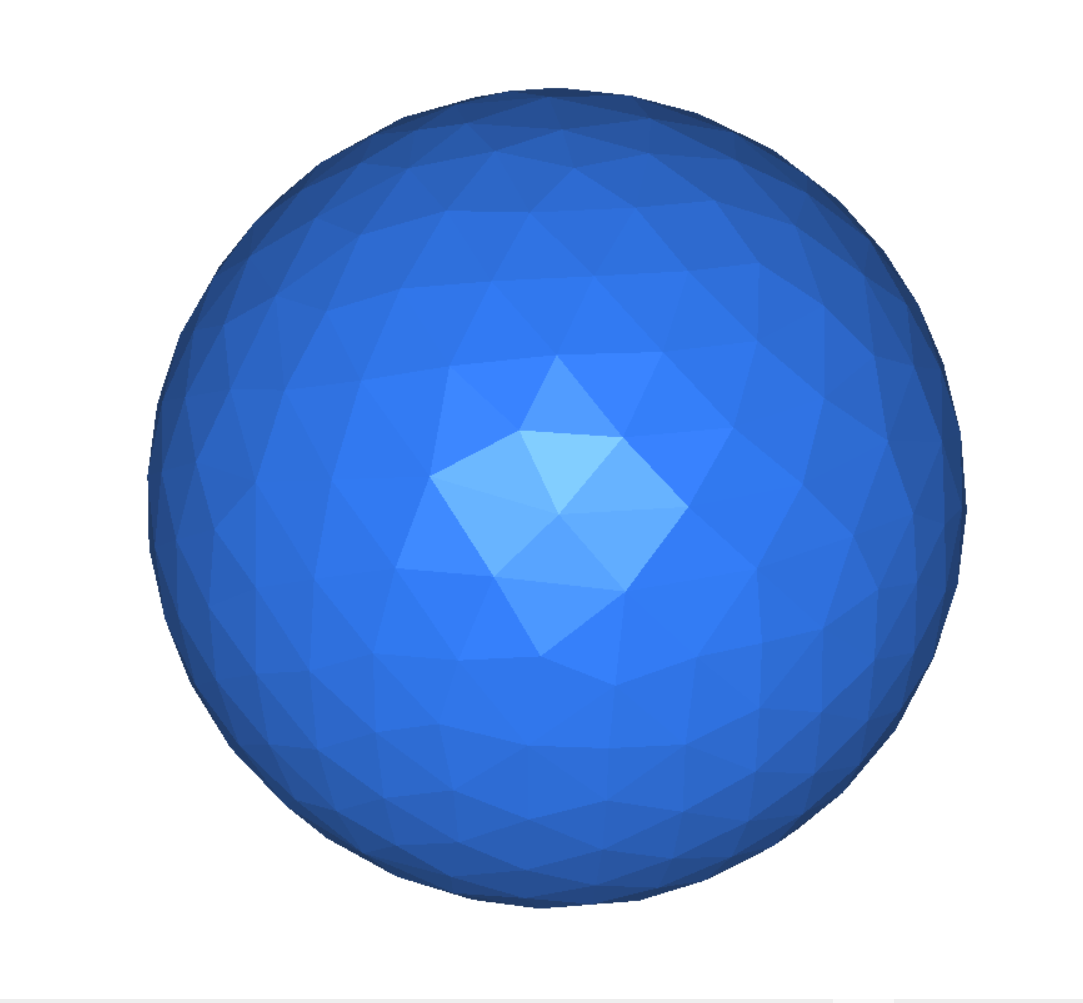
\includegraphics[width=0.22\linewidth]{1st_scatterer} \label{fig:q1} }  
	\hspace{4ex}
	\subfigure[]{
		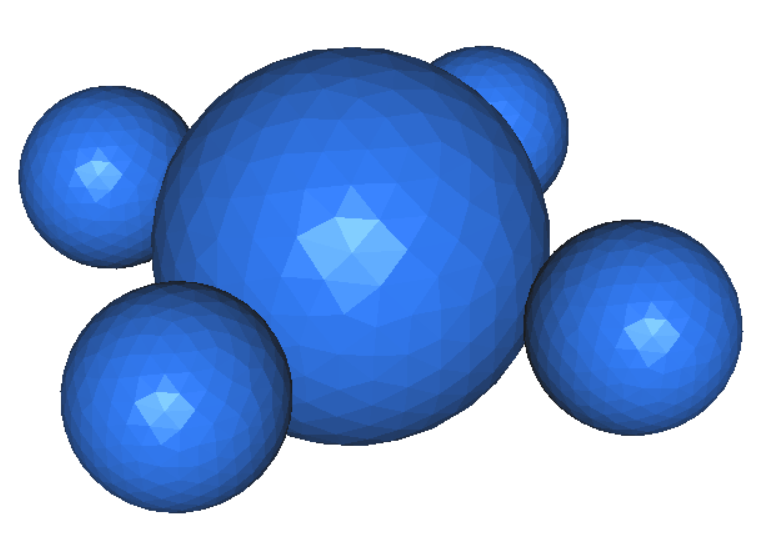
\includegraphics[width=0.25\linewidth]{2nd_scatterer} \label{fig:q2} }
	\hspace{4ex}
	\subfigure[]{ 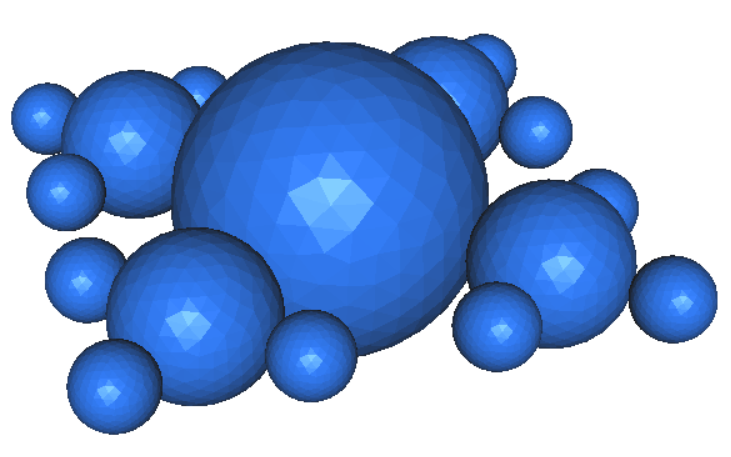
\includegraphics[width=0.3\linewidth]{3td_scatterer} \label{fig:q3}
	}  
	\caption{Eдиничная сфера (a) ; первая итерация - 5 сфер(b); вторая итерация - 17 сфер(c).} 
	\label{fig:qqq}
\end{figure} \\
\begin{flushleft}
	
После этого решим задачу дифракции одиночной сферы используя метод конечных элементов. Для этого наш объект заключим в сферическую область, в которой будут рассеиваться волны. Сразу определим, что внутри нашего объекта область заполнена диэлектриком, а его радиус будет в 10 раз меньше длины волны принимаемой для расчетов ($ \lambda = 1 $), а радиус сферической области в 4 раза больше (Рис.\ref{fig:ces1}). Так же стоит отметить, что на протяжении всей работы будет использоваться гармоническая зависимость $ e^{j \omega t} $, где $ j = \sqrt{-1} $. Далее найдем сечение рассеяния $ \sigma_s $ и сечение поглощения $ \sigma_a $, которое будет находиться на удалении $ \lambda = 3 $, с помощью действительной $ \varepsilon' $ и мнимой $ \varepsilon'' $ части диэлектрической проницаемости на основе коэффициентов преломления $ n' $ и $ n'' $. Сделаем тоже самое для всех трех случаев.  Для удобства поиска решения расчеты будем производить в декартовой системе координат. \\
\end{flushleft}

\begin{figure}[h!]
	\centering
	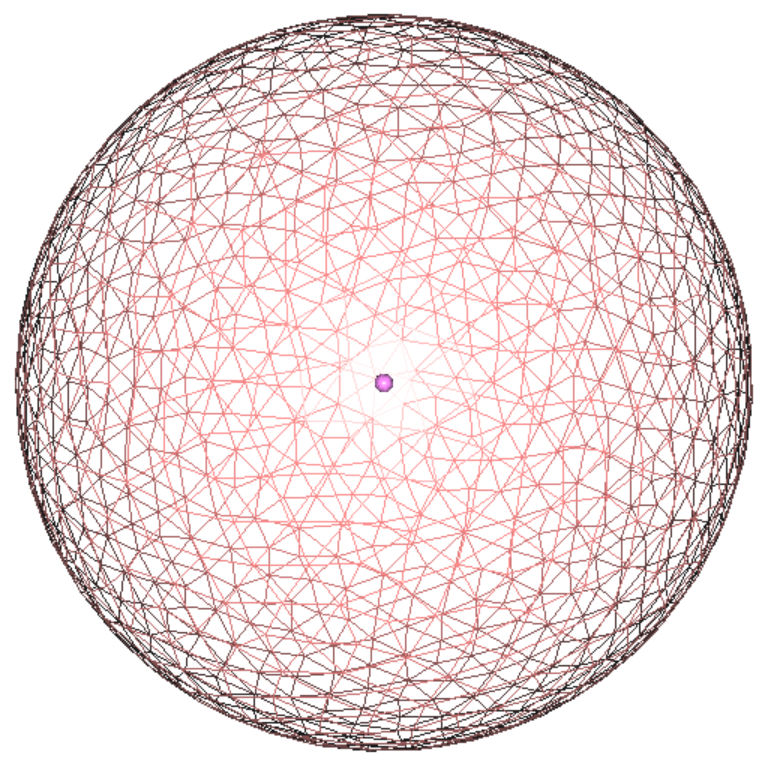
\includegraphics[width=0.5\linewidth]{ces1}
	\caption{}
	\label{fig:ces1}
\end{figure}
На Рис.~\ref{fig:q5} можно увидеть случай с 17 сферами, где в центре находится сам объект, окруженный сечением рассеяния, заключенный в сферическую область.\\
\begin{figure}[h!]
	\centering
	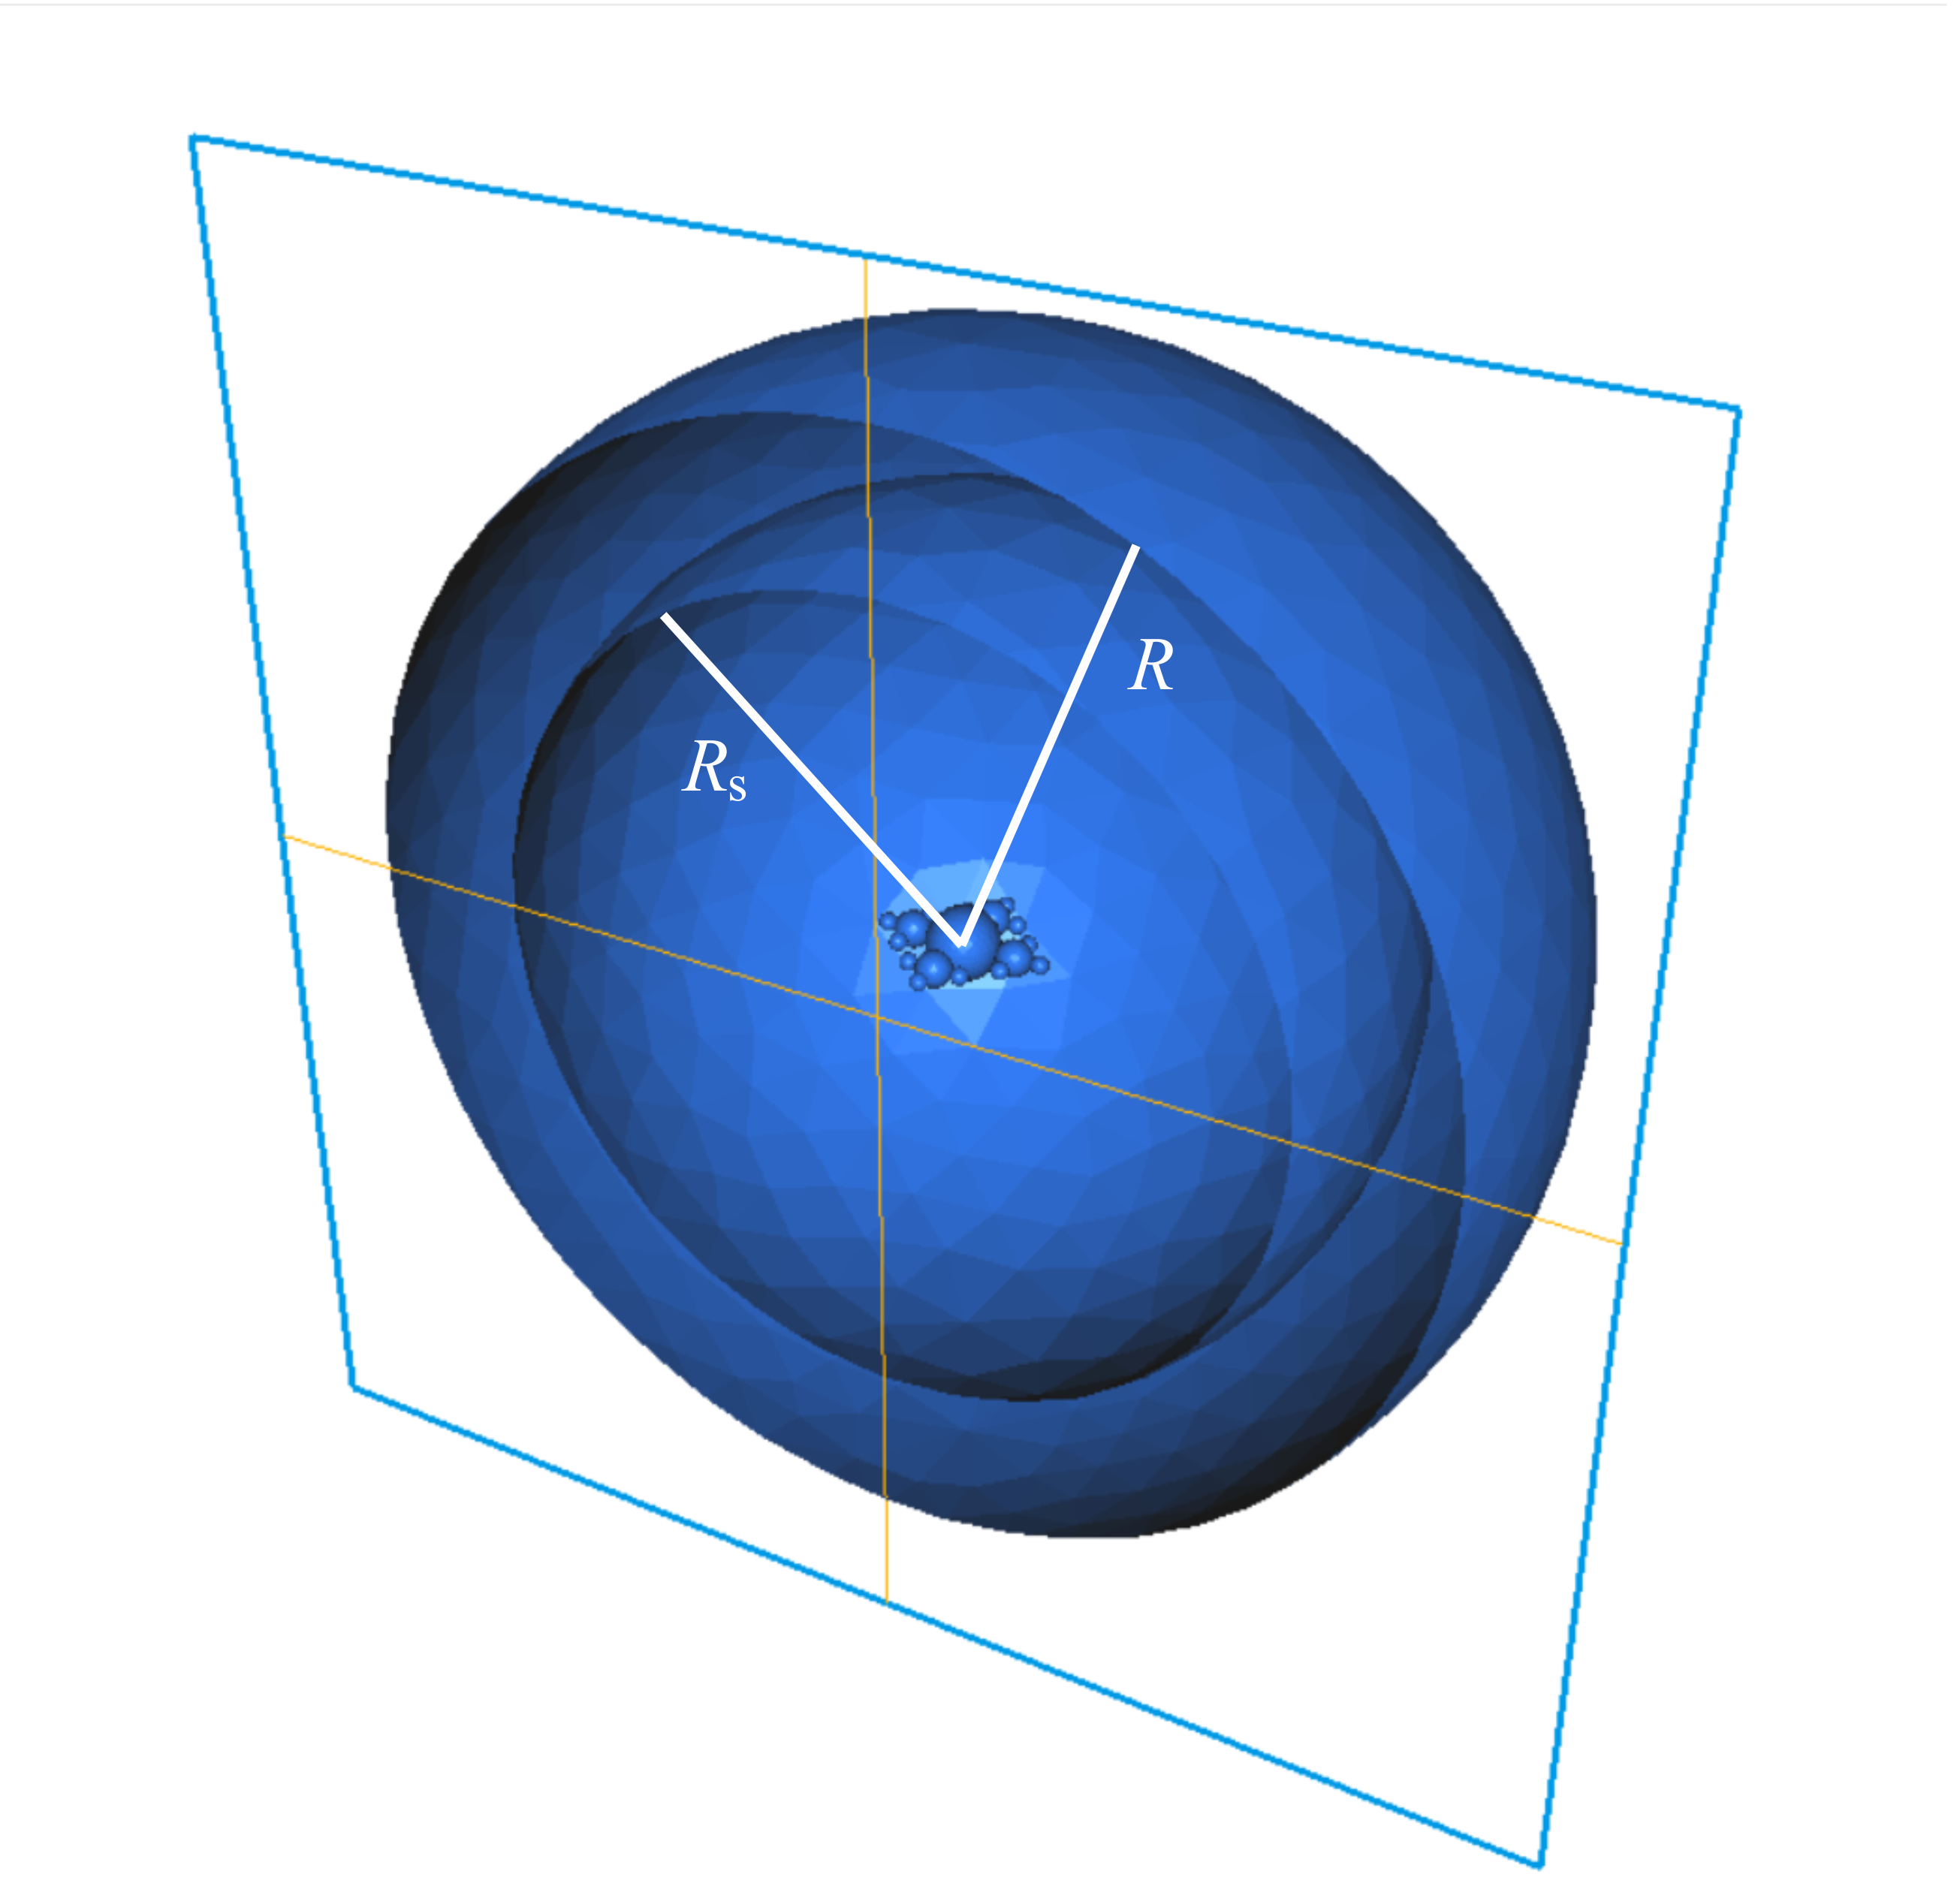
\includegraphics[width=0.6\linewidth]{3td_scattererAndOuterSpheres}
	\caption{}
	\label{fig:q5}
\end{figure}

\section{Описание метода решения задачи}
\begin{flushleft}
	Рассчеты для цилиндра будем производить в простейшем двумерном случае.
\end{flushleft}
\\
В начале запишем уравнение Максвелла: \\

\begin{center}
	$ 	\rm rot\vec{E} = -\dfrac{1}{c}\dfrac{\partial \vec{B}}{\partial t} $ 
\end{center}
\begin{center}
	$ 	\rm rot\vec{H} =\dfrac{4\pi}{c}\vec{j} + \dfrac{1}{c}\dfrac{\partial \vec{D}}{\partial t} $
\end{center}
\begin{center}
	$ 	div\vec{D} = 4\pi \rho $
\end{center}
	\begin{center}
		$ div \vec{B} = 0 $, где
	\end{center} 
\begin{center}
	$ \vec{H} = \vec{r}_{0}H_{0}\rm cos(\omega t - kz) $, и $ \varepsilon = 1 $ \\
\end{center}
При этом не забыв про материальные уравнения, которые описывают характеристики среды, в которой распространяется электромагнитная волна,а именно наличие диэлектриков ($ \varepsilon $), ферромагнетиков ($ \mu $), удельной проводимости ($ \gamma $):
\begin{center}
	$ \vec{D} = \varepsilon_{0} \varepsilon \vec{E} $
\end{center}
\begin{center}
	$ \vec{B} = \mu_{0} \mu \vec{H} $
\end{center}
\begin{center}
	$ \vec{j} = \gamma \vec{E} $
\end{center}
Где $ \varepsilon_{0} $ и $ \mu_{0} $ - соответственно электрическая и магнитная постоянные, $ \varepsilon $ и $ \mu $ - диэлектрическая и магнитная проницаемости, $ \gamma $ - удельная проводимость вещества. \\
А так же запишем уравнение Гельмгольца:
\begin{center}
	$ \Delta H_{z} + k^2H_{z} = 0 $ 
\end{center}\\
Из этого получаем : \begin{center}
	$ \rm rot\vec{H} = ik_{0}\vec{H} $
\end{center}
Отсюда выражаем  \vec{E}: \\
\begin{center}
	$\vec{E} = - \dfrac{i}{k_{0}} \rm rot\vec{H} = - \dfrac{i}{k_{0}}(\vec{x_{0}}\dfrac{\partial \vec{H_{z}}}{\partial y} - \vec{y_{0}}\dfrac{\partial \vec{H_{z}}}{\partial x}) 
	$
\end{center}

\begin{flushleft}
	А так же для $ E_{x} и E_{y} $ соответственно: \\
\end{flushleft}
\begin{center}
	$ E_{x} = - 
	\dfrac{i}{k_{0}}
	\dfrac{\partial\vec{H_{z}}}{\partial y} \\
	E_{y} = \dfrac{i}{k_{0}}
	\dfrac{\partial\vec{H_{z}}}{\partial x} \\ $
\end{center} \\
\begin{flushleft}
	Для условной поверхности S :
\end{flushleft} \\
\begin{center}
	$ [\vec{n}, \vec{x_{0}}E_{x} + \vec{y_{0}}E_{y}] = 0 $
\end{center}\\

\begin{flushleft}
	Таким образом получим интеграл:
\end{flushleft} \\

\begin{center}
	$ \int\limits_{V}^{} \Delta H_{z} \cdot wdv = - \int\limits_{V}^{}(\nabla H_{z}, \nabla w)dv +  \int\limits_{V}^{}(\nabla H_{z} \cdot w)dv
	$ \\
\end{center}

\begin{flushleft}
	Так как один из интегралов правой части: 
\end{flushleft}
\begin{center}
	$  \int\limits_{V}^{}(\nabla H_{z} \cdot w)dv $
\end{center} \\
\begin{flushleft}
	Соответственно равен: 
\end{flushleft}\\
\begin{center}
	$\int\limits_{V}^{}(\nabla H_{z} \cdot w)dv = \oint\limits_{S}^{} \nabla H_{z}  wds \cdot \vec{n} = 0 $ \\
\end{center}
\\
\begin{flushleft}
	То граничные условия в нашей задаче задавать нет необходимости.
	Поэтому получим:
\end{flushleft} \\

\begin{center}
	$ \nabla H_{z} = \vec{x}_{0} \dfrac{\partial\vec{H_{z}}}{\partial x} - \vec{y}_{0}
	\dfrac{\partial\vec{H_{z}}}{\partial y} $
	\\
\end{center}
\begin{flushleft}
	Cоответственно используя нормали $n_{x}$ и $n_{y}$  запишем искомое уравнение:
\end{flushleft} \\
\begin{center}
	$ \vec{n}\nabla H_{z} = \dfrac{\partial\vec{H_{z}}}{\partial n} = 
	n_{x}\dfrac{\partial\vec{H_{z}}}{\partial x} +
	n_{y}\dfrac{\partial\vec{H_{z}}}{\partial y} $
\end{center}

 \\
\begin{flushleft}
	Теперь решим ту же самую задачу, но уже точным методом. Для этого в начале найдем уравнения, которые нам понадобятся для решений:
\end{flushleft}\\

\begin{center}
	$ \vec{H} = \vec{r_{0}}H_{z}
\vec{H_{z}} = 1.e^{-ik_{0}x} = e^{-ik_{0}\rho \rm cos\varphi} = 
\sum\limits_{m=-\infty}^{\infty} J_{m}(k_{0}\rho)e^{-im(\varphi + \dfrac{\pi}{2})} =
\sum\limits_{m=-\infty}^{\infty} (-i)^{m}J_{m}(k_{0}\rho)e^{-im\varphi}
$
\end{center}\\

\begin{flushleft}
	Запишем уравнение Гельмгольца и оператор Лапласа в следующем виде:
\end{flushleft} \\
\begin{center}
	$ 
	\Delta_{\perp}H_{z} + k_{0}H_{z} = 0, \qquad
	\Delta_{\perp} = \dfrac{1}{\rho}
	\dfrac{\partial}{\partial \rho} 
	(\rho \dfrac{\partial}{\partial \rho}) + 
	\dfrac{1}{\rho^{2}}
	\dfrac{\partial^{2}}{\partial \varphi^{2}} 
	$
\end{center}
\\
\begin{flushleft}
	Получим:
\end{flushleft} \\
$$ \dfrac{\partial^{2}}{\partial \rho^{2}}H_{z}  +
\dfrac{1}{\rho}\dfrac{\partial}{\partial \rho}H_{z} +
\dfrac{1}{\rho^{2}}\dfrac{\partial^{2}}{\partial \varphi^{2}}H_{z}+
k_{o}^{2}H_{z} = 0 $$
\\
\begin{flushleft}\\
	
	Представим $ H_{z} $ как некую $ R(\rho) $ и $ \Phi(\varphi) $:\quad
	$ H_{z} = R(\rho)\Phi(\varphi) $, \qquad тогда : \\
\end{flushleft}

$$
&& \Phi^{\prime\prime}(\varphi) + m^2\Phi(\varphi) = 0 \quad -> \Phi(\varphi) = e^{-im\varphi} \\
&& R^{\prime\prime}(\rho) + \dfrac{1}{\rho} R^{\prime} + 
(k_{0}^{2} - \dfrac{m^{2}}{\rho^{2}})R = 0
$$ 
\\
\begin{flushleft}
	Отсюда получим, что :
\end{flushleft} \\
$$
R(\rho) = A_{1}H_{m}^{(1)}(k_{0}\rho) + A_{2}H_{m}^{(2)}(k_{0}\rho)
$$
\\
Однако \quad  $ A_{1} = 0 $, \quad так как
$\quad \lim\limits_{\rho -> \infty}\sqrt{\rho}
(\dfrac{\partial H_{m}^{(2)}}{\partial \varphi \rho} + ik_{0}H_{m}^{(1)} )
$ \\

\begin{flushleft}
	В таком случае у нас остается: \\
\end{flushleft}

$$
H_{z} = \sum_{m=-\infty}^{\infty}A_{2m}H_{m}^{(2)}(k_{0}\rho)e^{-im\varphi}
$$
\\
\begin{flushleft}
	Граничные условия:
\end{flushleft} 
\begin{center}
	$ E_{\varphi}|_{\rho=a} = 0 $
\end{center}\\
\begin{flushleft}
	Тогда:
\end{flushleft}
$$
\vec{E}^{(s)} = - \dfrac{i}{k_{0}\varepsilon} \rm rot\vec{H}^{(s)} = - \dfrac{i}{k_{0}} \dfrac{1}{\rho}
\begin{vmatrix}
\\\vec{\rho}_{0}& \;\rho \vec{\varphi}_{0}& \; \vec{z}_{0} \\
\dfrac{\partial }{\partial \rho}& \; 
\dfrac{\partial }{\partial \varphi}&\; 
\dfrac{\partial }{\partial z} \\
H_{\rho}&\; \rho H_{\varphi}&\; H_{z}^{(s)}
\end{vmatrix}
= \dfrac{i}{k_{0}} \dfrac{1}{\rho}(\vec{\rho_{0}} 
\dfrac{\partial H_{z}}{\partial \rho} - \rho\vec{\varphi}_{0}
\dfrac{\partial H_{z}^{(s)}}{\partial \rho}})
$$\\
$$
E_{\varphi}^{(s)} = \dfrac{i}{k_{0}}
\dfrac{\partial }{\partial \rho} \sum_{m=-\infty}^{\infty} A_{2m}H_{m}^{(2)}(k_{0}\rho)e^{-im\varphi} =
\dfrac{i}{k_{0}} \sum_{m=-\infty}^{\infty}A_{2m} 
\dfrac{\partial }{\partial \rho}
(H_{m}^{(2)}(k_{0}\rho))e^{-im\varphi}
= \\$$
\begin{center}
$$
i\sum_{m=-\infty}^{\infty}A_{2m}H_{m}^{(2)}^{\prime}(k_{0}\rho)e^{-im\varphi}
$$
\end{center}

\begin{flushleft}
Исходя из граничных условий для падающей и отраженной волны:
\end{flushleft} \\
$$
E_{\varphi}|_{\rho=a} = (E_{\varphi}^{(i)} + E_{\varphi}^{(s)})|_{\rho=a} = \sum_{m=-\infty}^{\infty}
((-i)^{m}J_{m}^{\prime}(k_{0}\rho) + A_{2m}H_{m}^{(2)}^{\prime}(k_{0}\rho))e^{-im\varphi}|_{\rho=a} = 0 \\
$$
\begin{flushleft}
Получим искомое выражение:
\end{flushleft}
$$
(-i)^{m}J_{m}^{\prime}(k_{0}a) + A_{2m}H_{m}^{(2)}^{\prime}(k_{0}a) = 0\\ $$
\begin{center}
$$
A_{2m} = (-i)^{m} \dfrac{J_{m}^{\prime}(k_{0}a)}
{H_{m}^{(2)}^{\prime}(k_{0}a)}
$$\\
\end{center}
\newpage
Теперь нам необходимо записать уравнение, с помощью которого мы и будем производить расчеты полей. Для этого обратимся к рис.1.
\\
\begin{figure}[h]
	\centering
	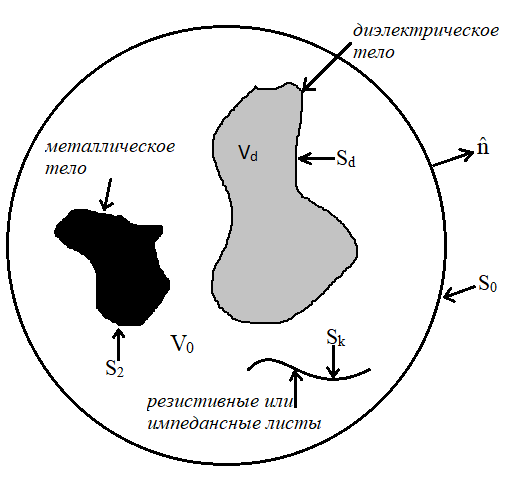
\includegraphics[width=0.6\linewidth]{tes2}
	\caption{}
	\label{fig:fr}
\end{figure}
\\
Вычислительная область ($ V_{0} $) ограничена поверхностью ($ S_{0} $) и может содержать различные рассеивающие объекты, такие как неоднородные диэлектрики ($ V_{d} $), металлические тела ($ S_{2} $) и резистивные или импедансные листы ($ S_{k} $).\\
Метод конечных элементов позволяет легко моделировать рассеиватели произвольной формы и неоднородные области, не предъявляя жестких требований к их форме, размеру и составу.  \\
Ввиду того, что наш интерес ограничен рассеянием, плотности электрического и магнитного тока будут равны нулю.
С учетом граничных условий на рассеивателе (ях), следует рассмотреть его средневзвешенное значение, дающее так называемую слабую форму векторного волнового уравнения. Для векторной функции $ \vec{E^{'}} $ (1):\\
\begin{center}
	$ 	\iiint\limits_{V_{0}}^{} \left[ \nabla \times \left( \dfrac{1}{\mu_{r}}\nabla \times \vec{E}\right)\cdot \vec{E^{'}} - k_{0}^{2} \epsilon_{r}\vec{E} \cdot \vec{E^{'}} \right]d\upsilon = 0 $
\end{center}
Однако уравнение должно выполняться для каждого из малых объемов, а не в каждой точке $ V_{0} $. Из-за двойного завитка, прямое численное решение уравнения (1) требует расширения $ \vec{E} $ с помощью базисных функций $ S_{0} $ более высокого порядка, и мы также можем получить асимметричную систему. Чтобы избежать этих трудностей и облегчить соблюдение граничных условий, традиционный подход состоит в том, чтобы использовать первую векторную идентичность Грина и переписать формулу: \\
\begin{center}
	$ 	\iiint\limits_{V_{0}}^{} \left[ \dfrac{1}{\mu_{r}}(\nabla \times \vec{E}) \cdot (\nabla \times \vec{E^{'}}) - k_{0}^{2} \epsilon_{r}\vec{E} \cdot \vec{E^{'}} \right]d\upsilon - jk_{0}Z_{0} \oiint (\hat{n} \times \vec{H}) \cdot \vec{E^{'}}ds = 0,$
\end{center}\\
где $ \vec{H} $ - полное магнитное поле, удовлетворяющее уравнению Максвелла $ \nabla \times \vec{E} - jk_{0}Z_{0}\vec{H}  $.\\
Уравнение (№) является слабой формой векторного волнового уравнения. Мы можем решить его численно для $ \vec{E} $, дискретизировав объем $ V_{0} $ и расширив $ \vec{E} $ подходящим, скажем, линейным расширением внутри каждого из подобъемов $V_{e}$. \\
Также необходимо обеспечить соблюдение всех необходимых граничных условий в пределах $V_{0}$ и на $S_{0}$, что подразумевает исключение $\vec{H}$, связав его с $\vec{E}$. \\
Учитывая, что наш интерес заключается в получении рассеяния тела, освещаемого плоской волной, $S_{0}$ служит только в качестве искусственной поверхности для завершения бесконечной вычислительной области. В самом деле, если $S_{0}$ находится далеко от рассеивателя, мы можем тогда вызвать условие излучения Зоммерфельда (2): \\
\begin{center}
	$ jk_{0}Z_{0}\hat{r} \times \vec{H}^{scat} = jk_{0}\hat{r} \times \hat{r} \times \vec{E}^{scat} $ \\
	\begin{center}
связав $ \vec{H} $ и $ \vec{E} $, где $ \hat{r} $ - нормаль к сферической поверхности $ S_{0} $ и \\
		$ \vec{H}^{scat} = \vec{H} - \vec{H}^{inc},\quad \vec{E}^{scat} = \vec{E} - \vec{E}^{inc}$
	\end{center}\\
Обозначим рассеянные поля, связанные с возбуждением плоской волны ($ \vec{E}^{inc} $, $ \vec{H}^{inc} $).
\end{center}
Очевидно, что требование, чтобы $ S_{0} $ располагалась далеко от рассеивателя, значительно увеличивает вычислительный объем, что приводит к непрактично большим системам при дискретизации уравнения. Это побудило к использованию поглощающих граничных условий более высокого порядка, которые можно наносить на поверхность, находящуюся в ближней зоне рассеивателя, без существенного снижения точности решения.Их целью является устранение обратных отражений от $ S_{0} $. \\
Они обеспечивают приблизительную связь между $\vec{E}$ и $\vec{H}$ на поверхности $ S_{0} $, которую мы получаем, предполагая расширение поля в обратных степенях r, радиальное расстояние от центра $S_{0}$. Если поглощающие граничные условия аннулируют первые (2m + 1) обратные степени r, то их называют поглощающие граничные условия m-го порядка.
Поглощающие граничные условия нулевого порядка являются условием излучения Зоммерфельда, приведенным в формуле (2), а их вектор второго порядка имеет вид(3):\\
\begin{center}
	$ -jk_{0}Z_{0}\hat{n} \times \vec{H}^{scat} = jk_{0}\vec{E}_{t}^{scat} + \beta \nabla \times [\hat{n}(\nabla \times \vec{E}^{scat})_{n}] + \beta\nabla_{t} (\nabla \cdot \vec{E}_{t}^{scat})$.
\end{center} \\
В этом уравнении $ \hat{n} $ обозначает внешнюю нормаль к $S_{0}$, $\beta = 1/{2[jk_{0} + (1/r)]}$, а нижние индексы t и n обозначают тангенциальную и нормальную компоненты для $ S_{0} $ соответственно. 
Поглощающие граничные условия (уравнение (3)) были получены для сферической поверхности $ S_{0} $, однако, они хорошо работают, когда $ S_{0} $ является кусочно-плоской, чтобы она лучше соответствовала поверхности рассеивателя.
В этом случае $ \beta $ сводится к $ \beta = 1/(2jk_{0}) $.\\
Точно так же мы можем обобщить уравнение (2) для кусочно-плоских поверхностей, положив $ \hat{r} \rightarrow \hat{n} $.\\
Так же отметим, что, поскольку данные поглощающие граничные условия связывают рассеянные поля, лучше всего переписать формулу (1) в терминах рассеянных полей. Делая так, мы получаем (4): \\
\begin{center}
	$ \iiint\limits_{V_{0}}^{} \left[ \dfrac{1}{\mu_{r}}(\nabla \times \vec{E}^{scat}) \cdot (\nabla \times \vec{E^{'}}) - k_{0}^{2} \epsilon_{r}\vec{E}^{scat} \cdot \vec{E^{'}} \right]d\upsilon + 
	\iint\limits_{S_{0}}^{}  P(\vec{E}^{scat}) \cdot \vec{E^{'}}ds + 
	\iiint\limits_{V_{d}}^{} \left[ \dfrac{1}{\mu_{r}}(\nabla \times \vec{E}^{inc}) \cdot (\nabla \times \vec{E^{'}}) - k_{0}^{2} \epsilon_{r}\vec{E}^{inc} \cdot \vec{E^{'}} \right]d\upsilon + 
	jk_{0}Z_{0}\iint\limits_{S_{d}}^{} \dfrac{1}{\mu_{r}}(\hat{n} \times \vec{H}^{inc}) \cdot \vec{E^{'}}ds = 0, $
\end{center}\\
в котором $P(\vec{E^{scat}})$ равно представлению в правой части уравнения (2), $ V_{d} $ - это объем, занимаемый диэлектриками, а $ S_{d} $ - это поверхность между диэлектрическими интерфейсами. Мы вывели последние два интеграла в формуле (4) снова вызвав первое векторное тождество Грина и отметим, что $ \vec{E^{inc}} $ удовлетворяет волновому уравнению вектора свободного пространства. Очевидно, что (4) относится только к неизвестным $ \vec{E^{scat}} $, и мы можем приступить к его решению.
\section{Тестирование численной схемы}
\begin{flushleft}
	Приступим к созданию трехмерной модели в программе FreeFem на основе полученных нами выше выражений.  Для этого выберем наиболее подходящий программный способ реализации 3D объектов, а так же сразу определим, что наш объект будет в виде сферы(у которой тут же зададим радиус и другие параметры). 
	\\
	Возьмем сферическую область, в которой будут рассеиваться волны и заключим в нее наш объект - сферу более маленького радиуса заполненного диэлектриком.
\end{flushleft} \\
\begin{flushleft}
	Определим параметры характеризующие наше поле,а именно:
\end{flushleft} \\
\begin{flushleft}
	$ \lambda = 10^{-6} $ - длина волны в вакууме в метрах \\
\end{flushleft}
\begin{flushleft}
	$ c = 299792458 $ - скорость света в вакууме \\
\end{flushleft}
\begin{flushleft}
	$ \mu = 4\pi 10^{-7} $ - магнитная проницаемость в свободном пространстве \\
\end{flushleft}
\begin{flushleft}
	$ \varepsilon = \dfrac{\mu}{c^{2}} $ - диэлектрическая проницаемость в свободном пространстве \\
\end{flushleft}
\begin{flushleft}
	$ Z = \sqrt{\dfrac{\mu}{\varepsilon}} $ - импеданс свободного пространства \\
\end{flushleft}
\begin{flushleft}
	$ n = 2 $ - показатель преломления сферы \\
\end{flushleft}
\begin{flushleft}
	Радиус внутренней сферы (нашего объекта) зададим в 10 раз меньше длины волны принимаемой для расчетов ($ \lambda = 1 $), а радиус внешней сферы в 4 раза больше. Таким образом получим систему состоящую из двух сфер разного радиуса (одна внутри другой), взаимодействие между которыми опиcываются с помощью уравнений полученных ранее. Однако, прежде чем мы это сделаем, определим в программе область расчетов через радиус внутренней сферы, для случаев когда он больше или меньше радиуса применяемого для вычислений полей в ближней и дальней зоне. Необходимость этого заключается в том, что уравнение должно выполняться для каждого из малых объемов, а не в каждой точке, как было сказано ранее.
\end{flushleft}
\\ 
\begin{flushleft}
	Имея уравнения Лапласа:
\end{flushleft}
\\
\begin{center}
	$ \Delta \vec{E} + k^2\vec{E}=0 $
\end{center}
Опрелелим k для случаев:
\begin{center}
	k = 
	\begin{cases}
		1, & r > a\\
		n, & r < a ,\qquad $ где а - радиус малой сферы $
	\end{cases}
\end{center}
Далее добавим цикл, который ввиду гармонической зависимости от времени будет производить перерасчет данных и выводить результаты на экран, благодаря чему получится наглядная анимированная картина поля. А так же добавим возможность сохранения полученных данных для Matlab.\\
После того, как мы посчитали дифракцию на сфере, перейдем непосредственно к расчету сечения рассеяния и сечения поглощения.\\
Если на рассеивающий элемент падает волна с интенсивностью I(под интенсивностью понимается поток энергии через единичную площадку), то полная рассеянная мощность S будет пропорциональна I. Коэффициент пропорциональности между этими величинами $ \sigma_s $ называется полным сечением рассеяния и имеет размерность площади: \\
\begin{center}
	$ \sigma_s = \dfrac{S}{I} $
\end{center}
Так же введем понятие дифференциального сечения рассеяния
 $ \sigma_d(\theta,\varphi) $. Пусть $ dS(\theta, \varphi) $ - полная мощность, рассеянная в пределах телесного угла d$ \Omega $ в направлении $ (\theta,\varphi) $, тогда:
 \begin{center}
 	$ \sigma_d(\theta,\varphi) = \lim\limits_{d\Omega\rightarrow\infty} \dfrac{dS(\theta, \varphi)}{Id\Omega}. $s
 \end{center}
Приминительно к нашей задаче, это выражение примет вид:
\begin{equation}
\sigma_d(\theta,\varphi) = \lim\limits_{R\rightarrow\infty} \dfrac{R^2 S_r(\theta, \varphi)}{S_i}.
\end{equation}
Здесь вектор Пойнтинга падающей волны
\begin{equation}
{\vec S}_i = \dfrac{1}{2} \left[{\vec E}_i \times {\vec H}^*_i\right],
\end{equation}
радиальная компонента вектора Пойнтинга рассеянных волн
\begin{equation}
{S}_r = \dfrac{1}{2} \left[{\vec E}_s \times {\vec H}^*_s\right] \cdot {\vec \rho}_0
\end{equation}

В нашем случае при расчётах необходимо будет взять значения вектора Пойнтинга рассеянных волн на поверхности с фиксированным значением $R$ (приемлемо, если $R=3\lambda$, т.к. внешняя граница удалена на расстояние $4\lambda$).

Наиболее простой способ расчёта $S_r$ через компоненты в декартовой системе координат:
\begin{equation}
{S}_r = S_x \\rm cos(\varphi)\sin(\theta) + S_y \sin(\varphi)\sin(\theta) + S_z \\rm cos(\theta).
\end{equation}
Здесь
\begin{eqnarray}
& S_x = \dfrac{1}{2} \left(E_y H_z^* - E_z H_y^*\right),\nonumber\\
& S_y = \dfrac{1}{2} \left(E_z H_x^* - E_x H_z^*\right),\nonumber\\ & S_z = \dfrac{1}{2} \left(E_x H_y^* - E_y H_x^*\right).
\end{eqnarray}
Предполагается, что поля относятся к рассеянному полю (индеркс $s$ опущен).
Компоненты магнитного поля находим из уравнения Максвелла
\begin{equation}
{\vec H} = \dfrac{i}{k_0} {\rm \rm rot} \vec{E}.
\end{equation}

Полное сечение рассеяния находится как интеграл по полному телесному углу:
\begin{equation}
\sigma_s = \int_{4\pi} \sigma_d d\Omega.
\end{equation}

Сечение поглощения определяется как отношение полной мощности, теряемой первичной волной и преобразующейся в тепло в данной локальной области, к плотности потока энергии(интенсивности) в первичной волне, его находим как:
\begin{equation}
\sigma_a = \left(\int_V \dfrac{1}{2}\omega\varepsilon_0\varepsilon''|{\vec E}|^2 d V\right)/S_i.
\end{equation}
В случае, если падающее поле имеет единичную амплитуду ($|E_i|=1$):
\begin{equation}
\sigma_a = \int_V k \varepsilon''|{\vec E}|^2 d V.
\end{equation}
Здесь интегрирование проводится по области занятой диэлектрическим рассеивателем.

Вычисление действительной и мнимой частей диэлектрической проницаемости на основе коэффициента преломления будет выглядеть как:
\begin{equation}
\varepsilon' - i \varepsilon'' = (n'-i n'')^2.
\end{equation}
Отсюда действительная $ \varepsilon' $ и мнимая $ \varepsilon'' $ часть будут соответственно равны:
\begin{equation}
\varepsilon' = (n')^2 - (n'')^2,\quad \varepsilon'' = 2 n'n''.
\end{equation}

\section{Результаты численных расчётов}


